\documentclass{beamer}

\usepackage{graphicx}
\usepackage{adjustbox}
\usepackage{booktabs}

\title{Colorimetric Analysis Methodology}
\subtitle{Bacterial-Dye-Antibiotic Arrays}
\author{}
\date{\today}

\begin{document}

\frame{\titlepage}

\begin{frame}{Problem Setup}
\begin{itemize}
    \item \textbf{Objective}: Extract biological insights from a temporal sequence of colorimetric images ($0^{th}$ min to $25^{th}$ min).
    \item \textbf{System}: Bacterial-dye-antibiotic arrays (3x9 grid matrix).
    \item \textbf{Goal}: Determine the Minimum Inhibitory Concentration (MIC) and understand reaction kinetics.
    \item \textbf{Indicator}: Biological indicator dye transitions from blue (high $a^*$) to pink (higher $a^*$) as surviving bacteria metabolize it.
\end{itemize}
\end{frame}

\begin{frame}{Grid Detection \& Extraction}
\begin{itemize}
    \item \textbf{Histogram Projection}: Isolate bright sample wells from the dark tray background using grayscale conversion, thresholding, and morphology opening.
    \item \textbf{Peak Finding}: Identify well centers via prominent peaks in projected 1D histograms over X and Y axes.
    \item \textbf{Median Extraction}: Draw a 32-pixel radius circular mask at each identified well location and extract median intensity across RGB, CIELAB ($L^*a^*b^*$), and HSV color spaces.
\end{itemize}
\end{frame}

\begin{frame}{1. Temporal MIC Identification}
\begin{columns}
\begin{column}{0.5\textwidth}
\begin{itemize}
    \item \textbf{Method}: Automated kinetic slope detection on the $a^*$ (green-red) channel over time.
    \item \textbf{Threshold}: Monotonic linear regression slope ($m > 0.1$) indicates bacterial survival.
    \item \textbf{Result}: Column 5 identified as the MIC (last completely inhibited concentration).
\end{itemize}
\end{column}
\begin{column}{0.5\textwidth}
\centering
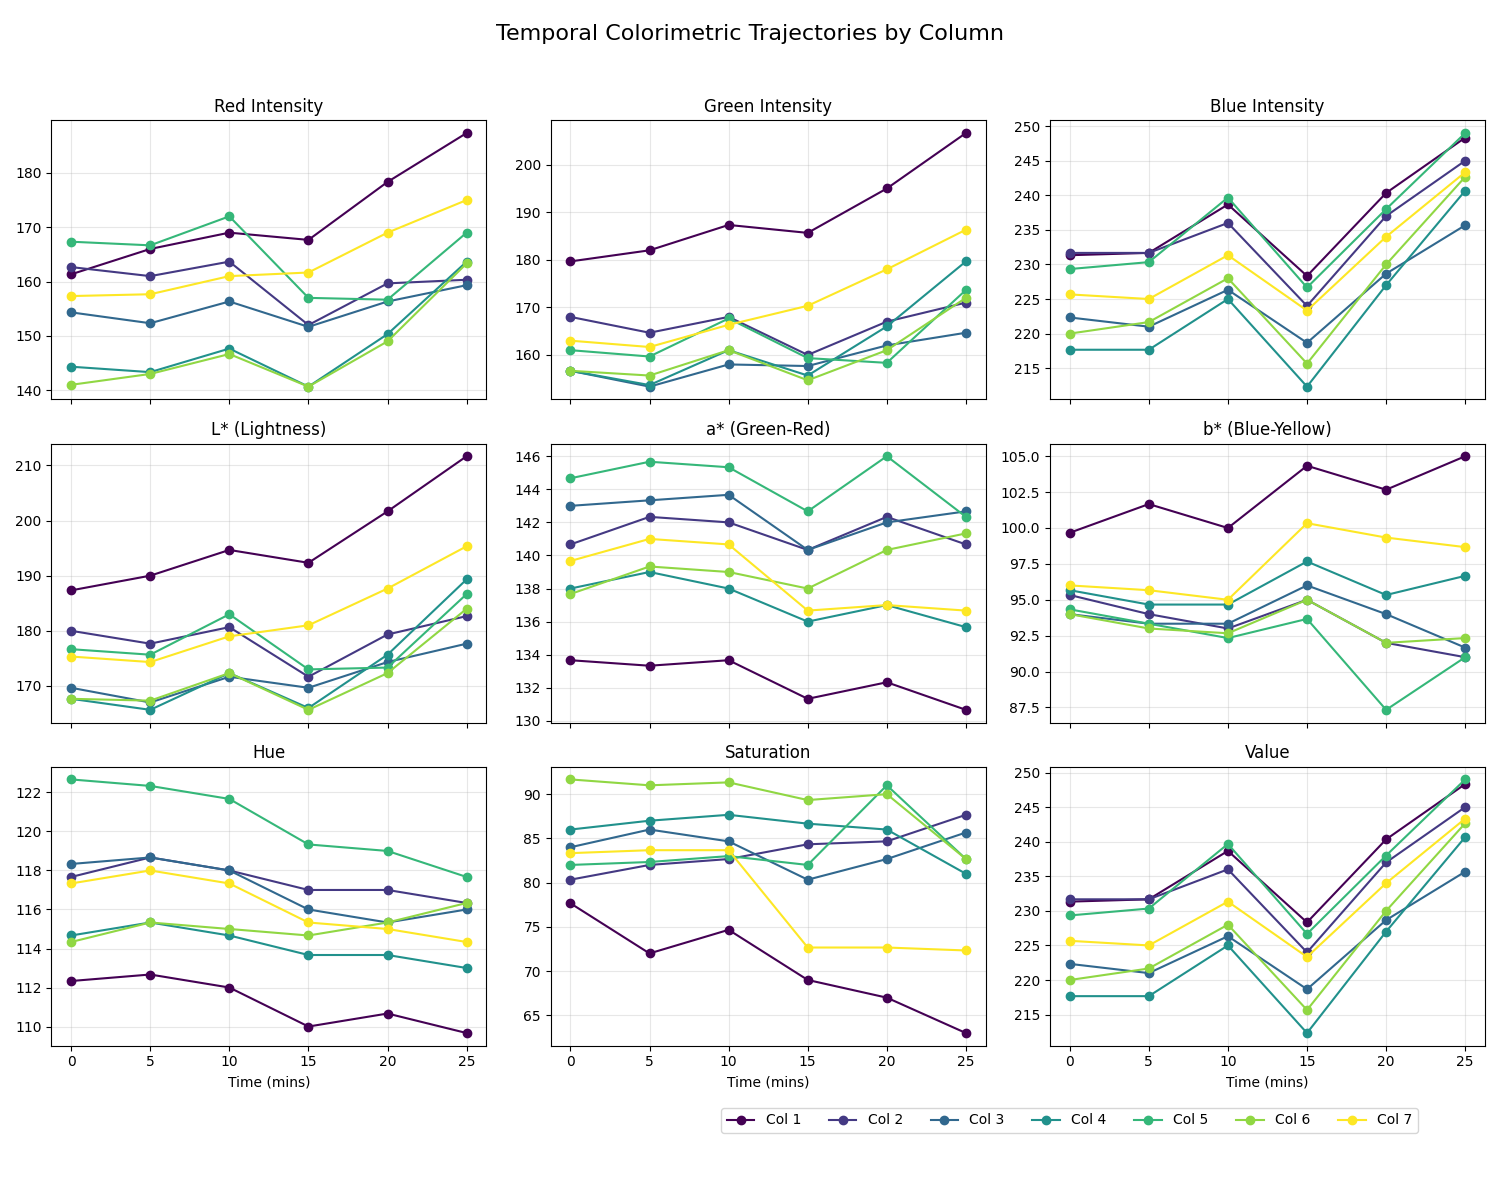
\includegraphics[width=\textwidth]{results/temporal/temporal_color_trends.png}
\end{column}
\end{columns}
\end{frame}

\begin{frame}{2. Principal Component Analysis (PCA)}
\begin{columns}
\begin{column}{0.5\textwidth}
\begin{itemize}
    \item \textbf{Purpose}: Dimensionality reduction of 9 distinct color features per sample per timepoint.
    \item \textbf{Inference}: Green (G), Lightness ($L^*$), and Saturation (S) channels carry the highest variance over the temporal sequence, more than traditional red-blue axes.
\end{itemize}
\end{column}
\begin{column}{0.5\textwidth}
\centering
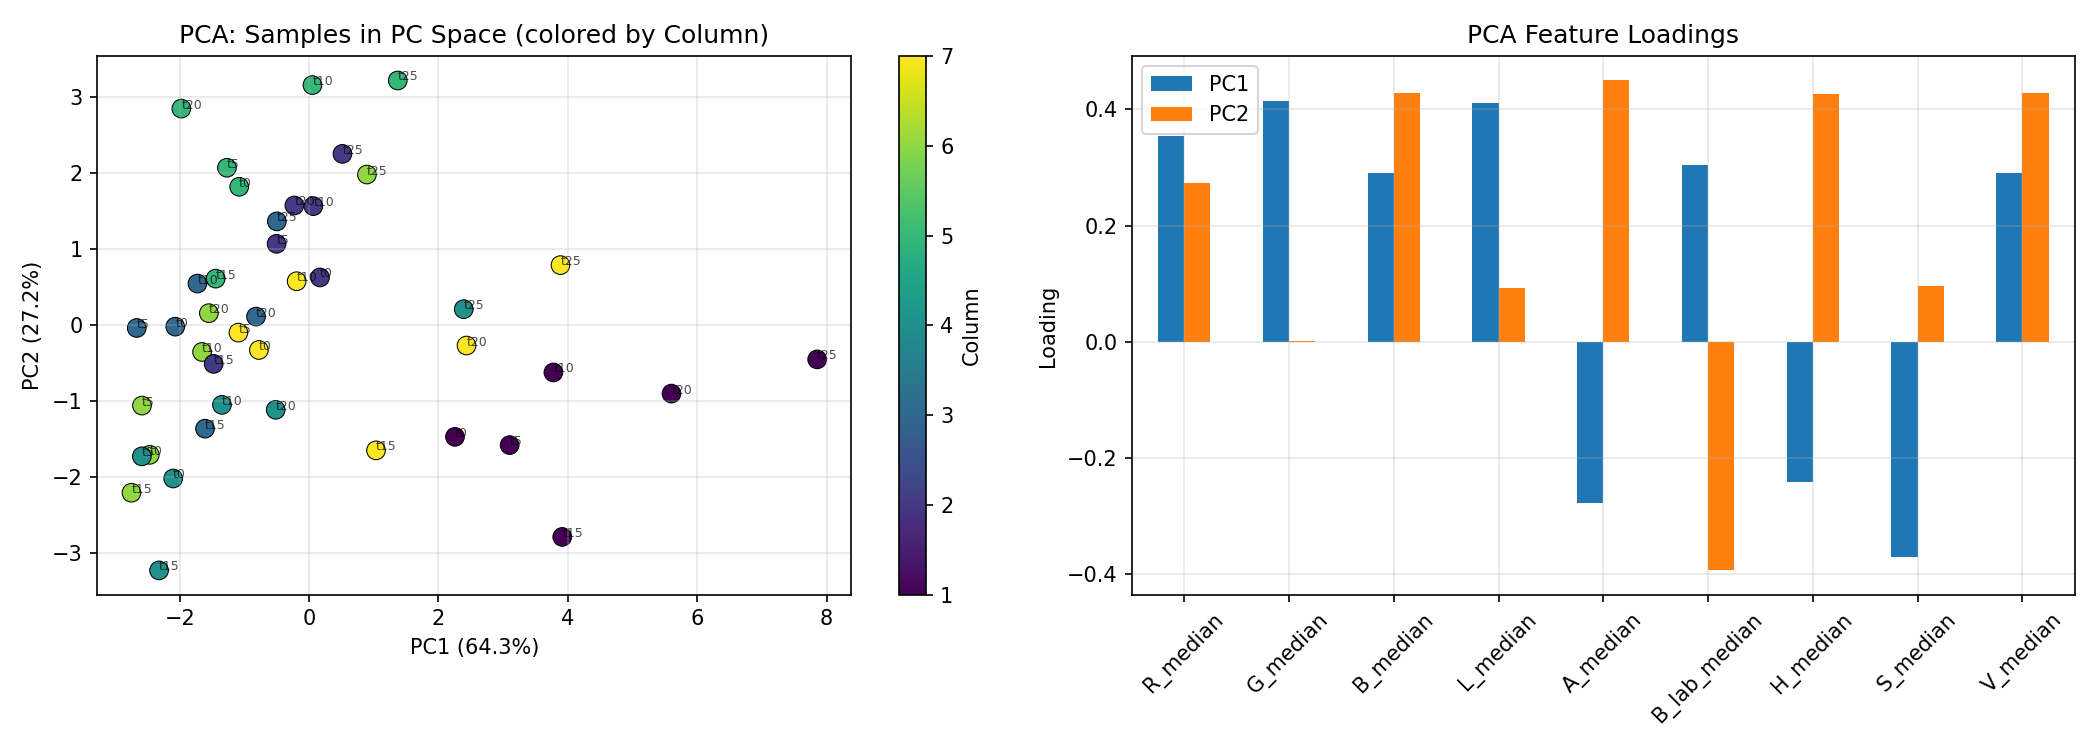
\includegraphics[width=\textwidth]{results/statistical/pca_analysis.png}
\end{column}
\end{columns}
\end{frame}

\begin{frame}{3. K-Means Behavioral Clustering}
\begin{columns}
\begin{column}{0.5\textwidth}
\begin{itemize}
    \item \textbf{Method}: Clustering flattened temporal trajectories ($K=3$).
    \item \textbf{Clusters identified}:
    \begin{enumerate}
        \item High Inhibition (Col 1)
        \item Transition/Stable Zone (Cols 2, 5, 7)
        \item High Activity (Cols 3, 4, 6)
    \end{enumerate}
    \item \textbf{Inference}: Response is not a smooth gradient but forms discrete "plateaus" of efficacy.
\end{itemize}
\end{column}
\begin{column}{0.5\textwidth}
\centering
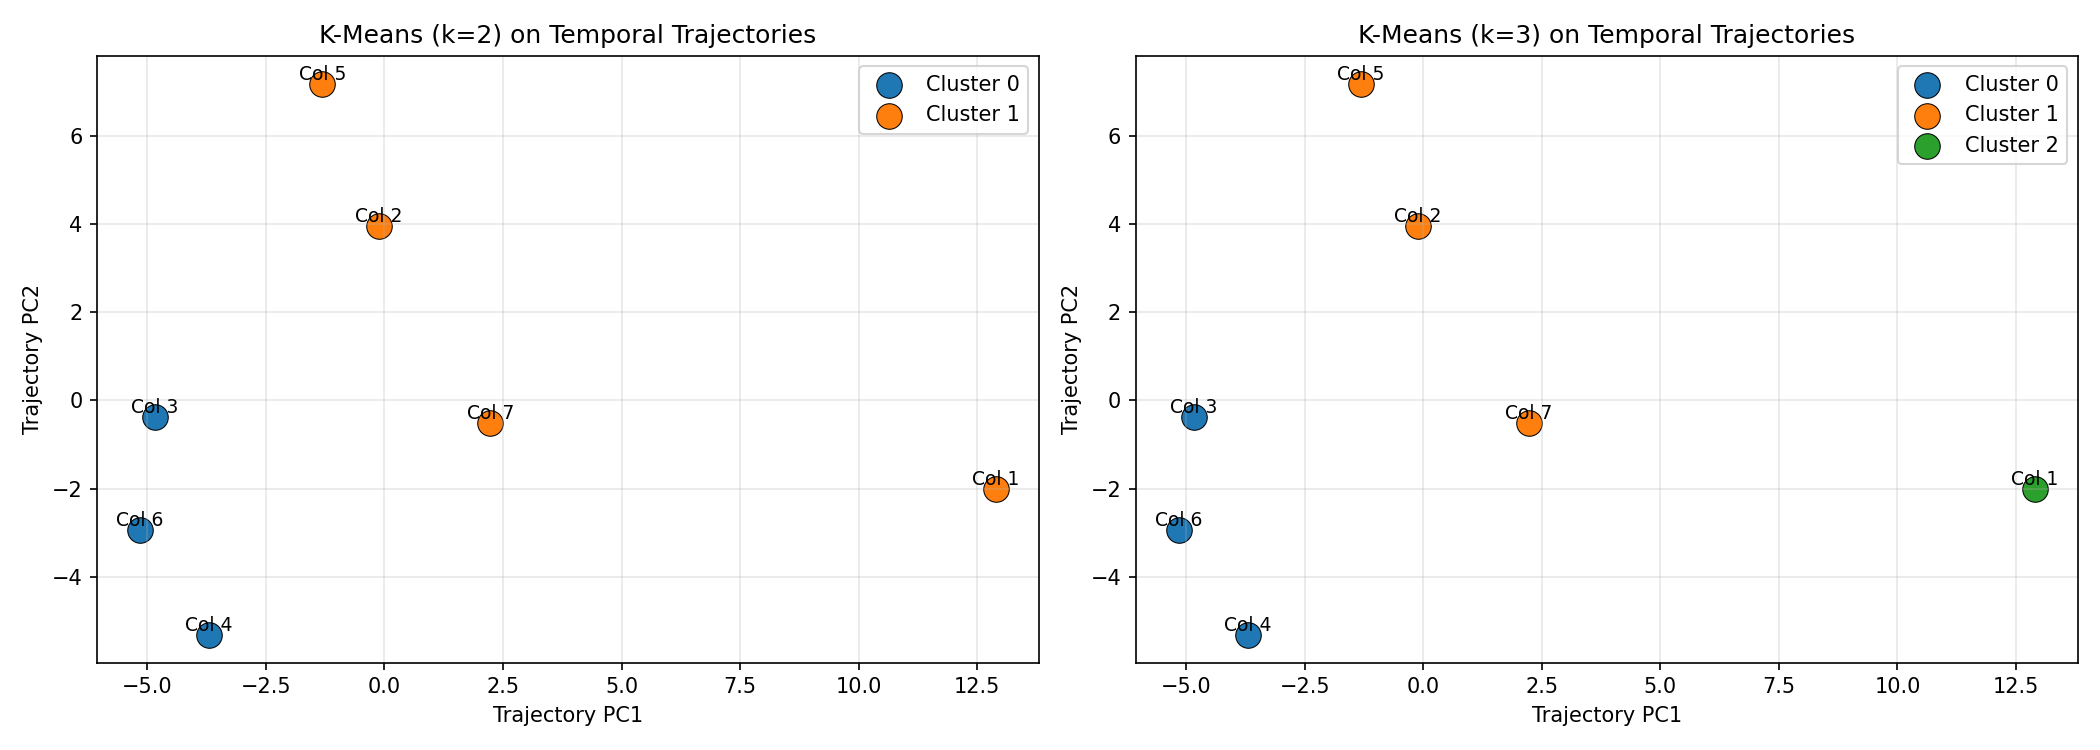
\includegraphics[width=\textwidth]{results/statistical/clustering_analysis.png}
\end{column}
\end{columns}
\end{frame}

\begin{frame}{4. Early Prediction \& Curvilinear Kinetics}
\begin{itemize}
    \item \textbf{Early Forecasting}: Logistic regression classifier achieved 85.7\% accuracy predicting final MIC outcome at $t=25$ using \textit{only} the initial $t=0$ image.
    \item \textbf{Curvilinear Kinetics}: Extracting $R^2$ exponential decay/growth coefficients using non-linear curve fits to overlying $a^*$ channel datapoints. Provides insight into deceleration rate and specific bacteriostatic/bactericidal mechanism.
\end{itemize}
\centering
\vspace{0.2cm}
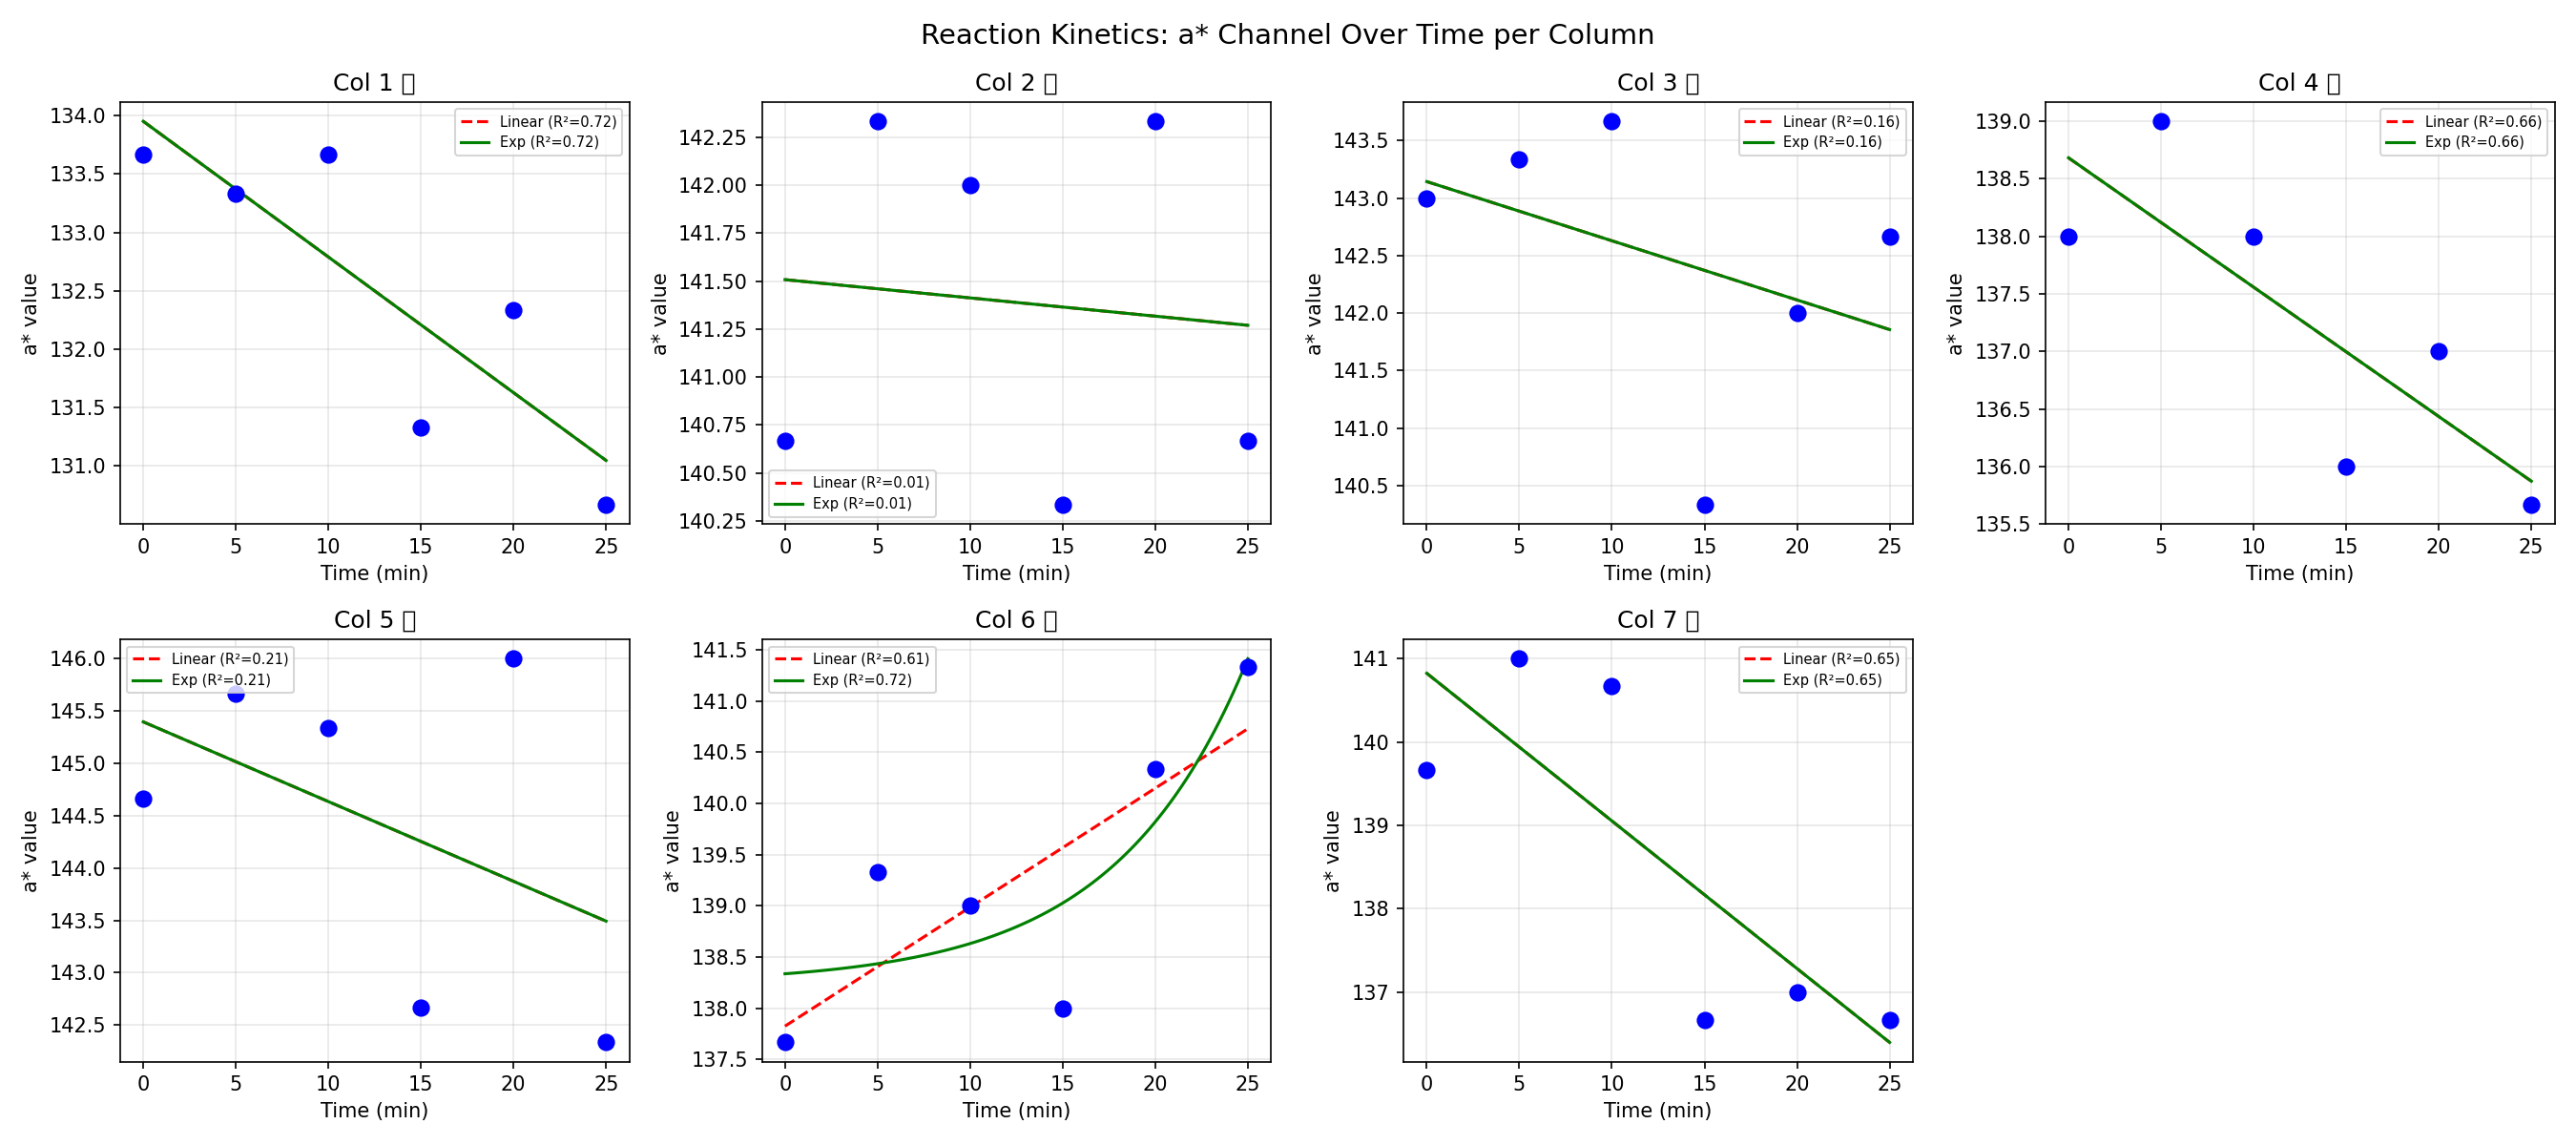
\includegraphics[width=0.6\textwidth, height=0.4\textheight, keepaspectratio]{results/statistical/kinetics_analysis.png}
\end{frame}

\begin{frame}{5. Replicate Consistency}
\begin{columns}
\begin{column}{0.5\textwidth}
\begin{itemize}
    \item \textbf{Method}: Calculated Coefficient of Variation (CV\%) across the 3 replicate rows.
    \item \textbf{Inference}: Assay layout is highly stable (CV 2.5\% - 5.5\%).
    \item \textbf{Anomaly}: Column 3 exhibited a variance spike (8.54\% CV), a hallmark of borderline transition to near-lethal antibiotic stresses.
\end{itemize}
\end{column}
\begin{column}{0.5\textwidth}
\centering
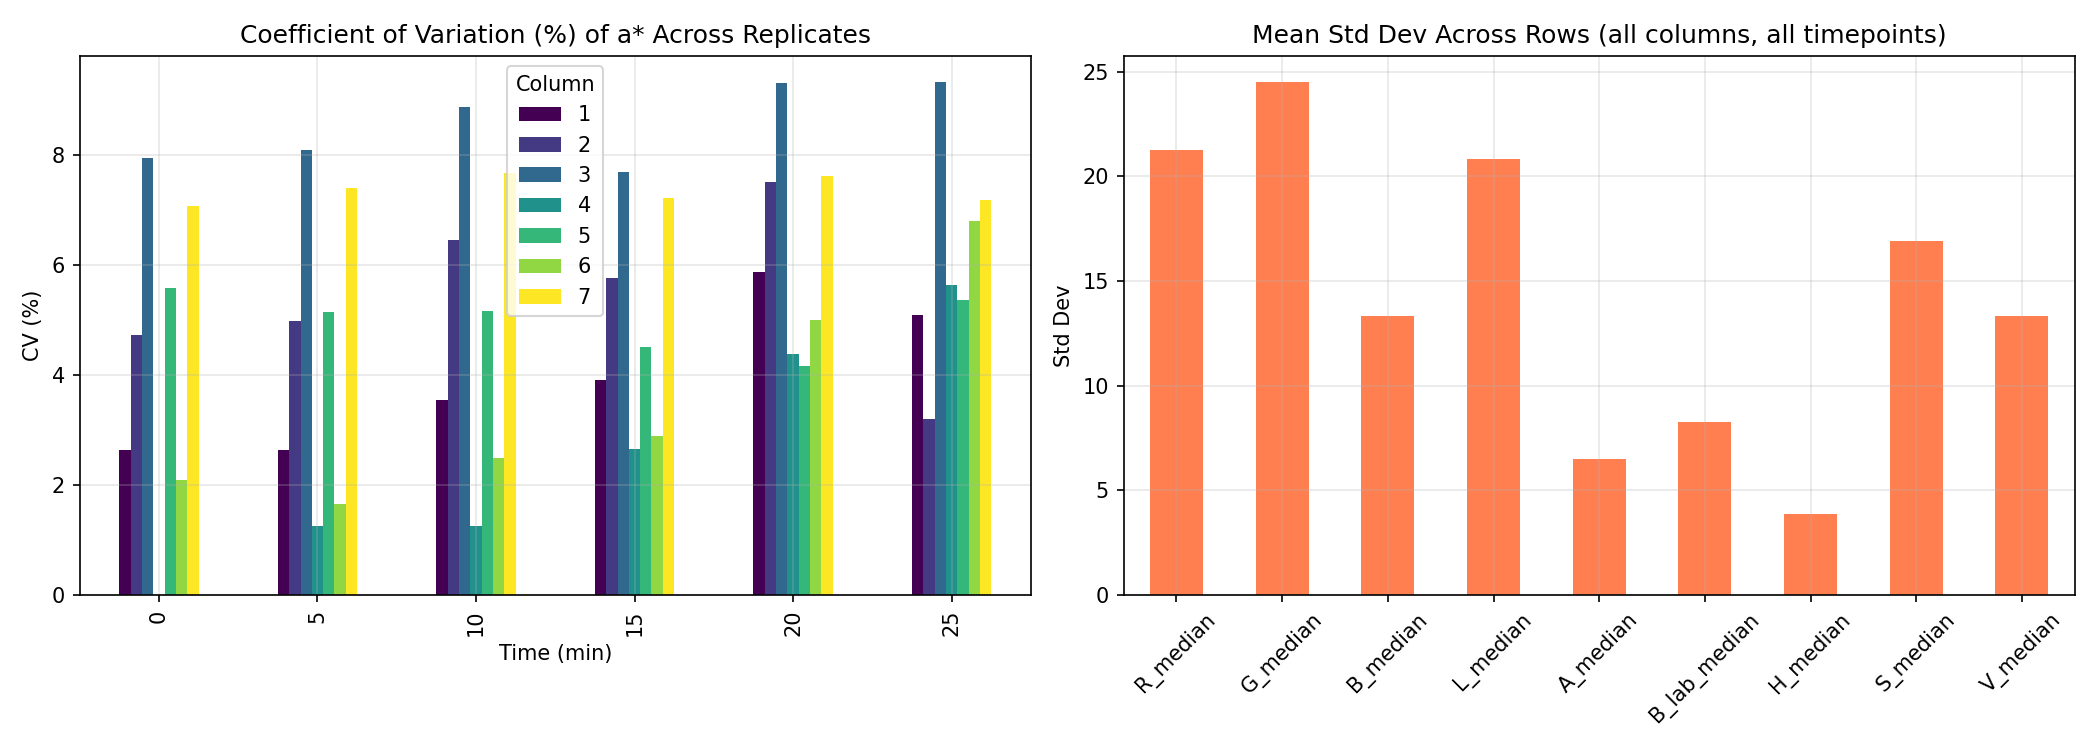
\includegraphics[width=\textwidth]{results/statistical/replicate_consistency.png}
\end{column}
\end{columns}
\end{frame}

\begin{frame}{6. Intra-Disk Region Detection}
\begin{columns}
\begin{column}{0.4\textwidth}
\begin{itemize}
    \item \textbf{Method}: K-Means clustering ($K=2$) spatially \textit{within} pixels of sample wells to isolate 'Reacted' (pink) from 'Unreacted' (blue).
    \item \textbf{Inference}: Growth isn't a uniform color fade. Pink region area percentage expands non-linearly, showing localized metabolic activity.
\end{itemize}
\end{column}
\begin{column}{0.6\textwidth}
\centering
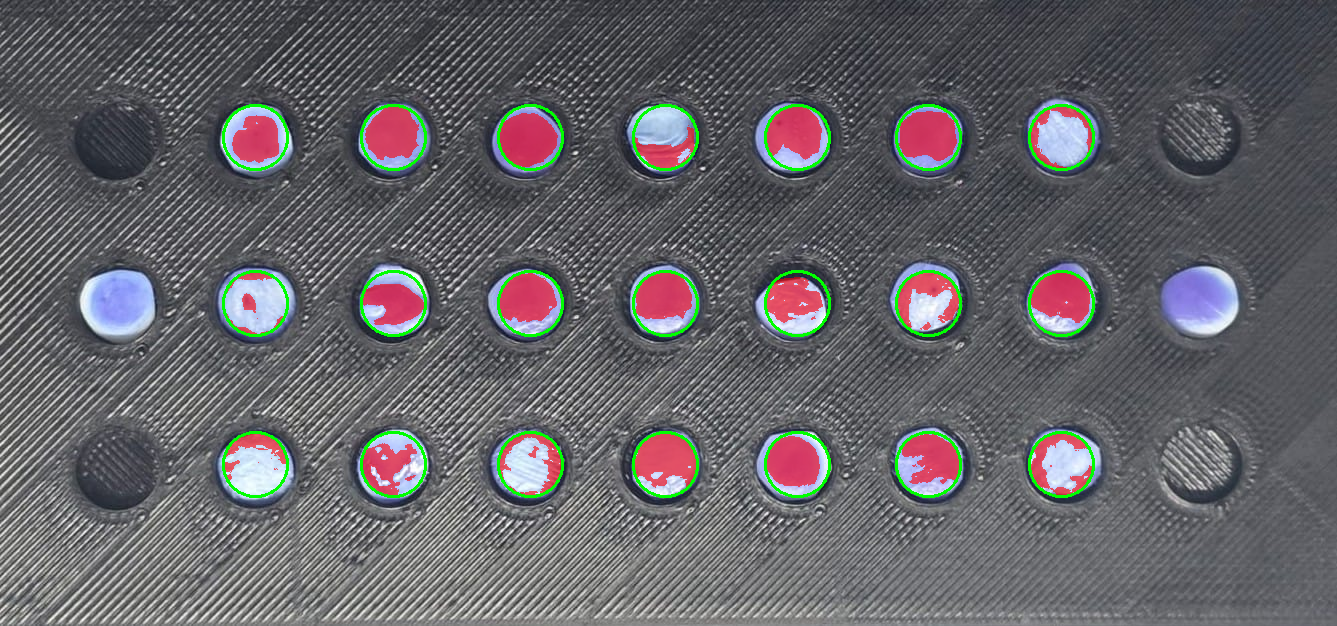
\includegraphics[width=\textwidth, height=0.4\textheight, keepaspectratio]{results/statistical/intra_disk_segmentation_t25.png}\\
\vspace{0.2cm}
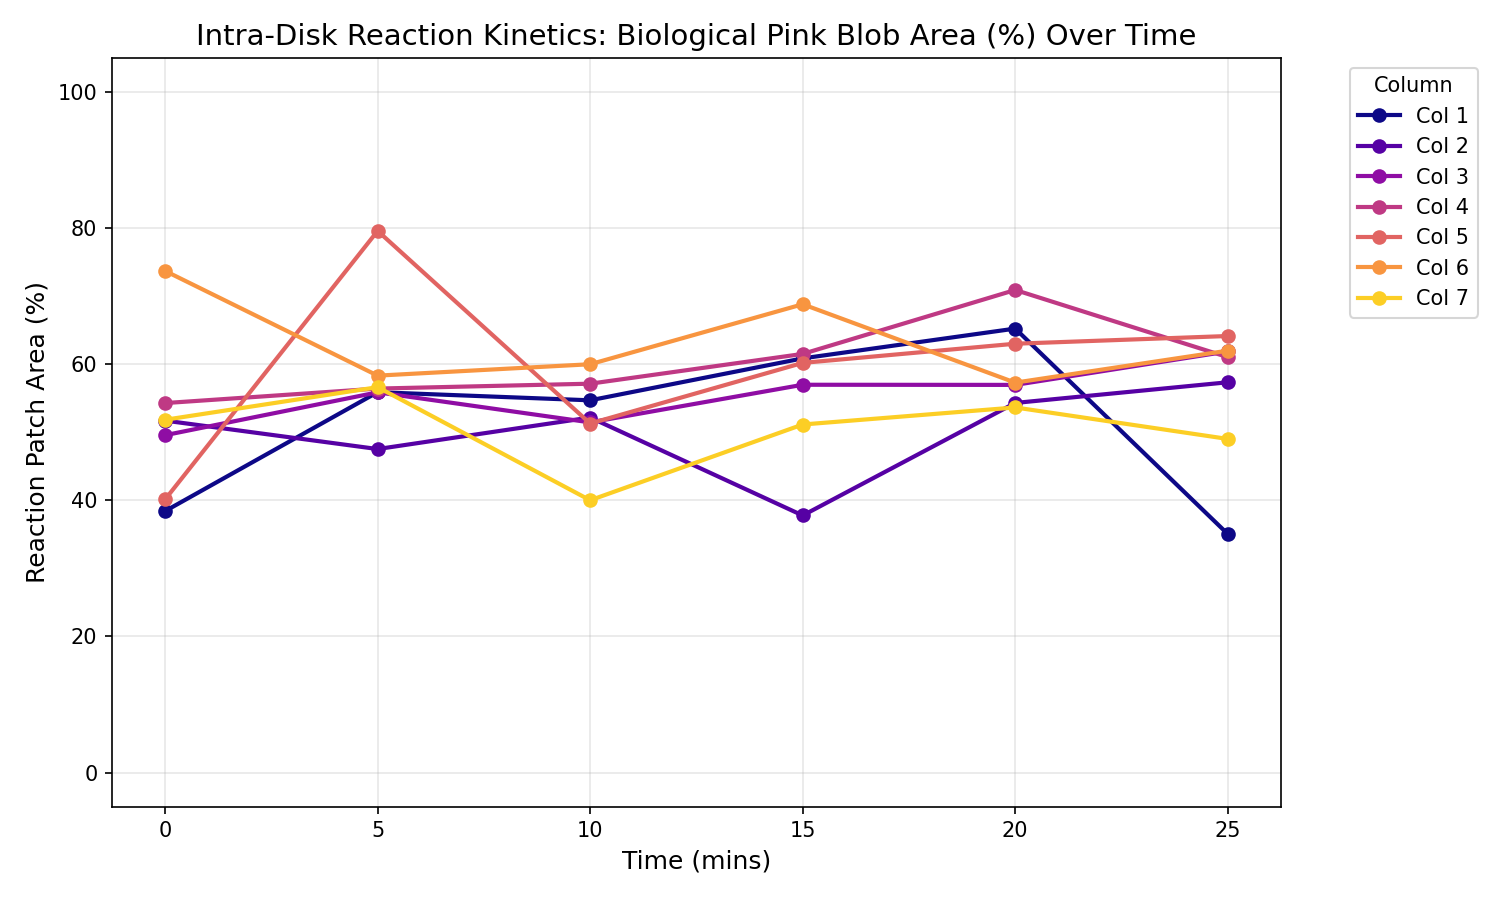
\includegraphics[width=\textwidth, height=0.4\textheight, keepaspectratio]{results/statistical/spatial_reaction_kinetics.png}
\end{column}
\end{columns}
\end{frame}

\begin{frame}{Conclusion}
\begin{itemize}
    \item Successfully automated MIC identification using robust, multi-channel colorimetric analysis.
    \item Advanced ML (PCA, K-Means) revealed deeper color channel insights \& non-linear behavioral responses.
    \item Spatial segmentation within discs proves growth is localized before diffusing.
    \item Early prediction models suggest feasibility of significantly reducing required incubation time.
\end{itemize}
\end{frame}

\end{document}
